
\documentclass[12pt,letterpaper]{article}
\usepackage{fullpage}
\usepackage[top=2cm, bottom=4.5cm, left=2.5cm, right=2.5cm]{geometry}
\usepackage{amsmath,amsthm,amsfonts,amssymb,amscd}
\usepackage{lastpage}
\usepackage{enumerate}
\usepackage{fancyhdr}
\usepackage{mathrsfs}
\usepackage{xcolor}
\usepackage{graphicx}
\usepackage{listings}
\usepackage{hyperref}
\usepackage{tikz}
\usepackage{xfrac}
\usepackage{nicefrac}
\usepackage{xcolor}

\allowdisplaybreaks


\usetikzlibrary{shapes.geometric,fit}
\usetikzlibrary{patterns}

\hypersetup{
  colorlinks=true,
  linkcolor=blue,
  linkbordercolor={0 0 1}
}

\setlength{\parindent}{0.0in}
\setlength{\parskip}{0.05in}

\newcommand\course{ECON 3213}
\newcommand\hwnumber{6}
\newcommand\NetIDa{dc3451}
\newcommand\NetIDb{David Chen}

\newcommand\R{\mathbb{R}}

\theoremstyle{definition}
\newtheorem*{statement}{Statement}
\newtheorem*{claim}{Claim}
\newtheorem*{theorem}{Theorem}

\newcommand{\contra}{\Rightarrow\!\Leftarrow}
\newcommand{\Lag}{\mathcal{L}}

\pagestyle{fancyplain}
\headheight 35pt
\lhead{\NetIDa}
\lhead{\NetIDa\\\NetIDb}
\chead{\textbf{\Large Problem Set \hwnumber}}
\rhead{\course \\ \today}
\lfoot{}
\cfoot{}
\rfoot{\small\thepage}
\headsep 1.5em

\begin{document}

\section*{Problem 1}

\subsection*{a}

\begin{center}
  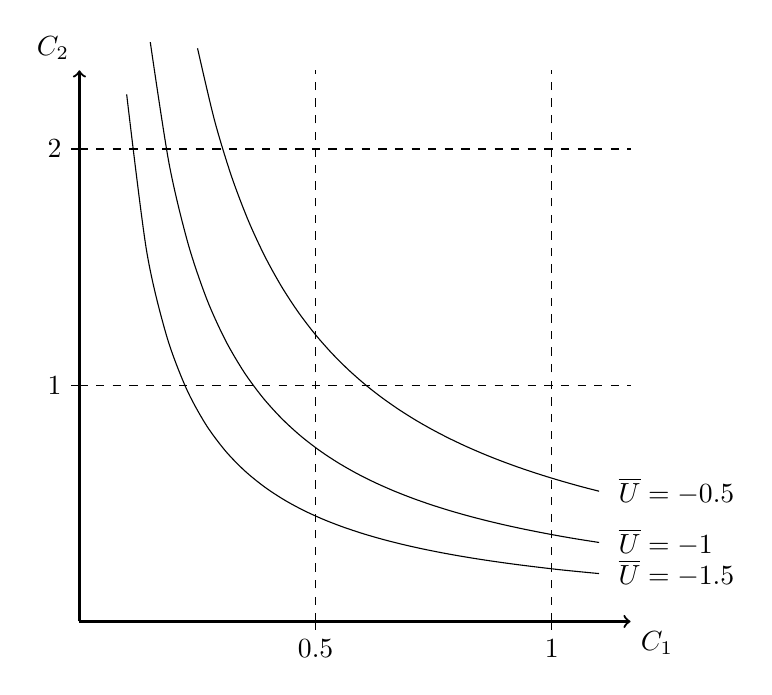
\begin{tikzpicture}[
    dot/.style={shape=circle, inner sep=2pt, draw, node contents=},
    circ/.style={shape=circle, inner sep=2pt, draw, fill}]
    \draw[thick,->] (0,0) -- (7,0) node[anchor=north west] {$C_1$};
    \draw[thick,->] (0,0) -- (0,7) node[anchor=south east] {$C_2$};
    \draw (3pt,6cm) -- (-3pt,6cm) node[anchor=east] {$2$}; 
    \draw (3pt,3cm) -- (-3pt,3cm) node[anchor=east] {$1$}; 
    \draw (3cm,3pt) -- (3cm,-3pt) node[anchor=north] {$0.5$};
    \draw (6cm,3pt) -- (6cm,-3pt) node[anchor=north] {$1$};
    \draw[domain=0.25:1.1,scale=6,smooth,variable=\x] plot ({\x},{0.5 * e^(-0.5) / \x}) node[label=right:{$\overline{U} = -0.5$}]{};
    \draw[domain=0.15:1.1,scale=6,smooth,variable=\x] plot ({\x},{0.5 * e^(-1) / \x}) node[label=right:{$\overline{U} = -1$}]{};
    \draw[domain=0.10:1.1,scale=6,smooth,variable=\x] plot ({\x},{0.5 * e^(-1.5) / \x}) node[label=right:{$\overline{U} = -1.5$}]{};

    \draw[dashed] (3,0) -- (3,7);
    \draw[dashed] (6,0) -- (6,7);
    \draw[dashed] (0,3) -- (7,3);
    \draw[dashed] (0,6) -- (7,6);
  \end{tikzpicture}
\end{center}

\subsection*{b}

\begin{align*}
  U &= \ln(C_1) + \ln(C_2) \\
  0 &= \frac{1}{C_1} + \frac{dC_2}{dC_1}\frac{1}{C_2} \\
  \frac{dC_2}{dC_1} &= -\frac{C_2}{C_1} 
\end{align*}

Computing the marginal rate of substitution,

\begin{align*}
  \frac{MU_1}{MU_2} &= \frac{1/C_1}{1/C_2} \\
                    &= \frac{C_2}{C_1} \\
                    &= -\frac{dC_2}{dC_1}
\end{align*}

\subsection*{c}

\[
  \frac{d^2C_2}{dC_1^2} = -\frac{C_1\frac{dC_2}{dC_1} - C_2}{C_1^2} =
  -\frac{-C_2 - C_2}{C_1^2} = \frac{2C_2}{C_1^2}
\]

Since we have that $C_2 > 0$, as we have a positive amount of consumption in
both periods to have real utility, and $C_1^2 > 0$ as well,
$\frac{d^2C_2}{dC_1^2} > 0$.

\subsection*{d}

Note that we have $C_2 = \frac{e^{U}}{C_1}$. Then, $\frac{dC_2}{dC_1} =
-\frac{e^U}{C_1^2} = -e^U$ when $C_1 = 1$.

For $U = -1.5$, $\frac{dC_2}{dC_1} = -e^{-1.5}$.

For $U = -1.0$, $\frac{dC_2}{dC_1} = -e^{-1.0}$.

For $U = -0.5$, $\frac{dC_2}{dC_1} = -e^{-0.5}$.

The reason that we see as utility diminishes the slope becomes flatter is that a
flatter slope represents a lower marginal rate of substitution, which in this
case is a lower willingness to trade $C_2$ for $C_1$. Since at lower utilities
with $C_1$ held constant we must have $C_2$ lower (since utility must be
increasing), and since preferences are convex, we would expect to see at lower
utilities a diminished willingness to trade $C_2$ for $C_1$, and thus a flatter slope.

\section*{Problem 2}

\subsection*{a}

Period 1:
\[
  C_1 + S_1 = Y_1
\]

where $S_1 = \sigma Y_1$ is the savings (or borrowing if $\sigma < 0$).

Period 2:

\[
  C_2  = Y_2 + S_1(1 + r)
\]

\subsection*{b}

\[
  C_1 + \frac{C_2}{1 + r} = Y_1 + \frac{Y_2}{1+r}
\]

\subsection*{c}

\[
  \max_{C_1, C_2}\{\sqrt{C_1} + \sqrt{C_2}\} \text{ such that } C_1 + \frac{C_2}{1 + r} = Y_1 + \frac{Y_2}{1+r}
\]

\subsection*{d}

Put $y = Y_1 + \frac{Y_2}{1+r}$.

\begin{align*}
  \mathcal{L}(C_1, C_2, \lambda) &= \sqrt{C_1} + \sqrt{C_2} - \lambda(C_1 + \frac{C_2}{1+r} - y) \\
  \frac{\partial \mathcal{L}}{\partial C_1} &= \frac{1}{2\sqrt{C_1}} - \lambda = 0 \\
  \frac{\partial \mathcal{L}}{\partial C_2} &= \frac{1}{2\sqrt{C_2}} - \frac{\lambda}{1+r} = 0 \\
  \frac{\partial \mathcal{L}}{\partial \lambda} &= C_1 + \frac{C_2}{1+r} - y = 0 \\
  \lambda &= \frac{1}{2\sqrt{C_1}} = \frac{1+r}{2\sqrt{C_2}} \\
  C_1 &= \frac{C_2}{(1+r)^2} \\
  y &= C_1 + (1+r)C_1 \\
  C_1 &= \frac{y}{2 + r} = \frac{Y_1}{2+r} + \frac{Y_2}{(1+r)(2+r)} = \frac{1}{2+r}(Y_1 + \frac{Y_2}{1+r})\\
  C_2 &= \frac{y(1+r)^2}{2+r} = (1+r)^2(\frac{Y_1}{2+r} + \frac{Y_2}{(1+r)(2+r)}) \\
                                 &= \frac{Y_1(1+r)^2}{2+r} + \frac{Y_2(1+r)}{2+r} = \frac{1}{2+r}(Y_1(1+r)^2 + Y_2(1+r)) \\
  S_1 &= Y_1 - C_1 \\
                                 &= \frac{1}{2+r}((1-r)Y_1 - \frac{Y_2}{1+r})
\end{align*}

\subsection*{e}

For $r = 0, Y_1 = Y_2 = 10$, one can note that this makes the problem symmetric in $C_1, C_2$. Then, $C_1 +
C_2 = Y_1 + Y_2 \implies C_1 = C_2 = \frac{1}{2}(Y_1 + Y_2) = 10, S_1 = 0$.

Anyway, substituting from above, we have that

\[
  C_1 = \frac{1}{2}(10 + 10) = 10, C_2 = \frac{1}{2}(10 + 10) = 10, S_1 = 10 - 10
  = 0
\]

For $r = 0.1,$
\[
  C_1 = \frac{1}{2.1}(10 + \frac{10}{2.1}) = 9.09, C_2 = 9.1(1.1)^2 = 11.01, S_1
  = 10 - 9.09 = 0.91
\]

\end{document}
% LocalWords:  nodecirc